\chapter{ Sprint 1 : Enhancements and Integrations}
\setcounter{secnumdepth}{0}

\section{Introduction}
In this chapter, we cover the first sprint of the Aermax project, focusing on the key enhancements and features we implemented to improve the platform.
\setcounter{secnumdepth}{2} 
\section{Major Features and Enhancements}
This section details the major features and enhancements introduced during the first sprint of the Aermax project. Each item listed in the sprint backlog was carefully selected to address critical needs and provide significant improvements to the platform's functionality and user experience.
\subsection{Sprint Backlog Detail}
Below is a detailed representation of our sprint backlog, showcasing the major tasks we committed to delivering in Sprint 1. We fixed around \textbf{26+ bugs, feature enhancements and new features }in Sprint 1. Below, we're going to share some of them. The biggest changes that we can discuss are highlighted below the blue colored line in the table.
\begin{longtable}{ | m{0.15\textwidth} | m{0.2\textwidth} | m{0.25\textwidth} | m{0.1\textwidth} | m{0.16\textwidth} | }
    \caption{Detailed Sprint Backlog} \\
    \hline
    \textbf{Type} & \textbf{Title} & \textbf{Description} & \textbf{Priority} & \textbf{Estimation} \\
    \hline
    \endfirsthead
    \hline
    \textbf{Type} & \textbf{Title} & \textbf{Description} & \textbf{Priority} & \textbf{Estimation} \\
    \hline
    \endhead
    \hline
    \endfoot
    \endlastfoot
    \rowcolor{blue!20} 
    Feature & Dynamic Equipment List & Develop a dynamic equipment list feature that organizes and manages equipment groups, ensuring each group and equipment item can be created, updated, and assigned to sub-companies and packets as needed. This feature aims to improve flexibility and ease of equipment management within the application. & High & 40h \\
    \hline
    \rowcolor{blue!20} Feature & Implement User Authentication System & Create a user authentication system enabling subcontractors to self-register, login, and manage passwords securely, allowing independent access to the platform's features. & High & 12h \\
    \hline
    \rowcolor{blue!20} 
    Enhancement & Adjust Feedback Notification & Enhance the feedback system to include notifications in Microsoft Teams, ensuring real-time updates . & Medium & 8h \\
    \hline
    Enhancement & Set Dynamic Project Status & Dynamically set project status based on packet statuses. & High & 5h \\
    \hline
    Enhancement & Add Field to User Edit & Include additional fields in the user edit form. & Medium & 2h \\
    \hline
    Feature & Set Default Calendar View & Remember last selection for default calendar view using localStorage. & Medium & 1h \\
    \hline
    Enhancement & Restrict Project Creation & Prevent subcontractors from creating new projects. & High & 1h \\
    \hline
    Enhancement & Remove Team Types & Remove unnecessary team types from the app to streamline functionality. & Low & 6h \\
    \hline
    Feature & Calendar View with New Filters & Implement new filters for the calendar view for better UX. & High & 40h \\
    \hline
    Feature & Implement Google Maps URL Generation & Generate Google Maps URLs for address visualization in subcompany user view. & Medium & 4h \\
    \hline
    Bug & Overhaul User Access Restrictions & Fix critical access restrictions and bugs for subcompany users. & High & 8h \\
    \hline
    \rowcolor{blue!20} 
    Feature & Overhaul the Role System & Revise the role system to clarify permissions and responsibilities. & High & 8h \\
    \hline
    Feature & Automate Username Generation & Auto-generate usernames during self-registration. & Medium & 16h \\
    \hline
    Feature & Remember Date Filters for Calendar & Implement a feature to remember date filters for the calendar. & Low & 3h \\
    \hline
    Feature & Overhaul the Project Status & Update project status features and adjust status enums and filters. & High & 3h \\
    \hline
    Bug & Fix Read-Only State of User Edit Form & Correct the issue with the user edit form being read-only for admins. & Medium & 4h \\
    \hline
    Bug & Remove Duplicate Aggregated Phases & Remove any duplicate instances of aggregated phases in the system. & High & 3h \\
    \hline
    \rowcolor{blue!20} Enhancement & Enhance Working Packets UI \& UX & Improve the UI and UX for working packets. & Medium & 16h \\
    \hline
\end{longtable}

\subsection{Dynamic Equipment List}
To effectively transition from a static to a dynamic equipment list, we need to carefully design the system architecture.

\subsubsection{Dynamic Equipment List Issues}
The Dynamic Equipment List feature was previously implemented as a static list, which required manual updates and did not reflect real-time changes to the equipment database. The key characteristics and drawbacks of the static implementation are outlined below:

\paragraph{Key Characteristics of the Static Implementation}
\begin{itemize}
    \item \textbf{Manual Updates:} The equipment list required manual updates.
    \item \textbf{Limited Flexibility:} The static list lacked flexibility and responsiveness to changes.
    \item \textbf{High Maintenance Overhead:} Frequent updates resulted in high maintenance overhead.
\end{itemize}

\paragraph{Drawbacks of the Static Implementation}
\begin{itemize}
    \item \textbf{Scalability:} As the number of equipment items grew, maintaining the static list became increasingly cumbersome.
    \item \textbf{Real-time Updates:} Changes to the equipment database were not immediately reflected in the list, leading to potential inconsistencies.
    \item \textbf{User Experience:} Users could not rely on the list for up-to-date information, impacting their ability to make informed decisions.
\end{itemize}

As illustrated in Figure \ref{fig:static_equipment_list}, subcontractors were limited to only checking the checkboxes for the available equipment.

\begin{figure}[H]
    \centering
    \resizebox{1\textwidth}{!}{
        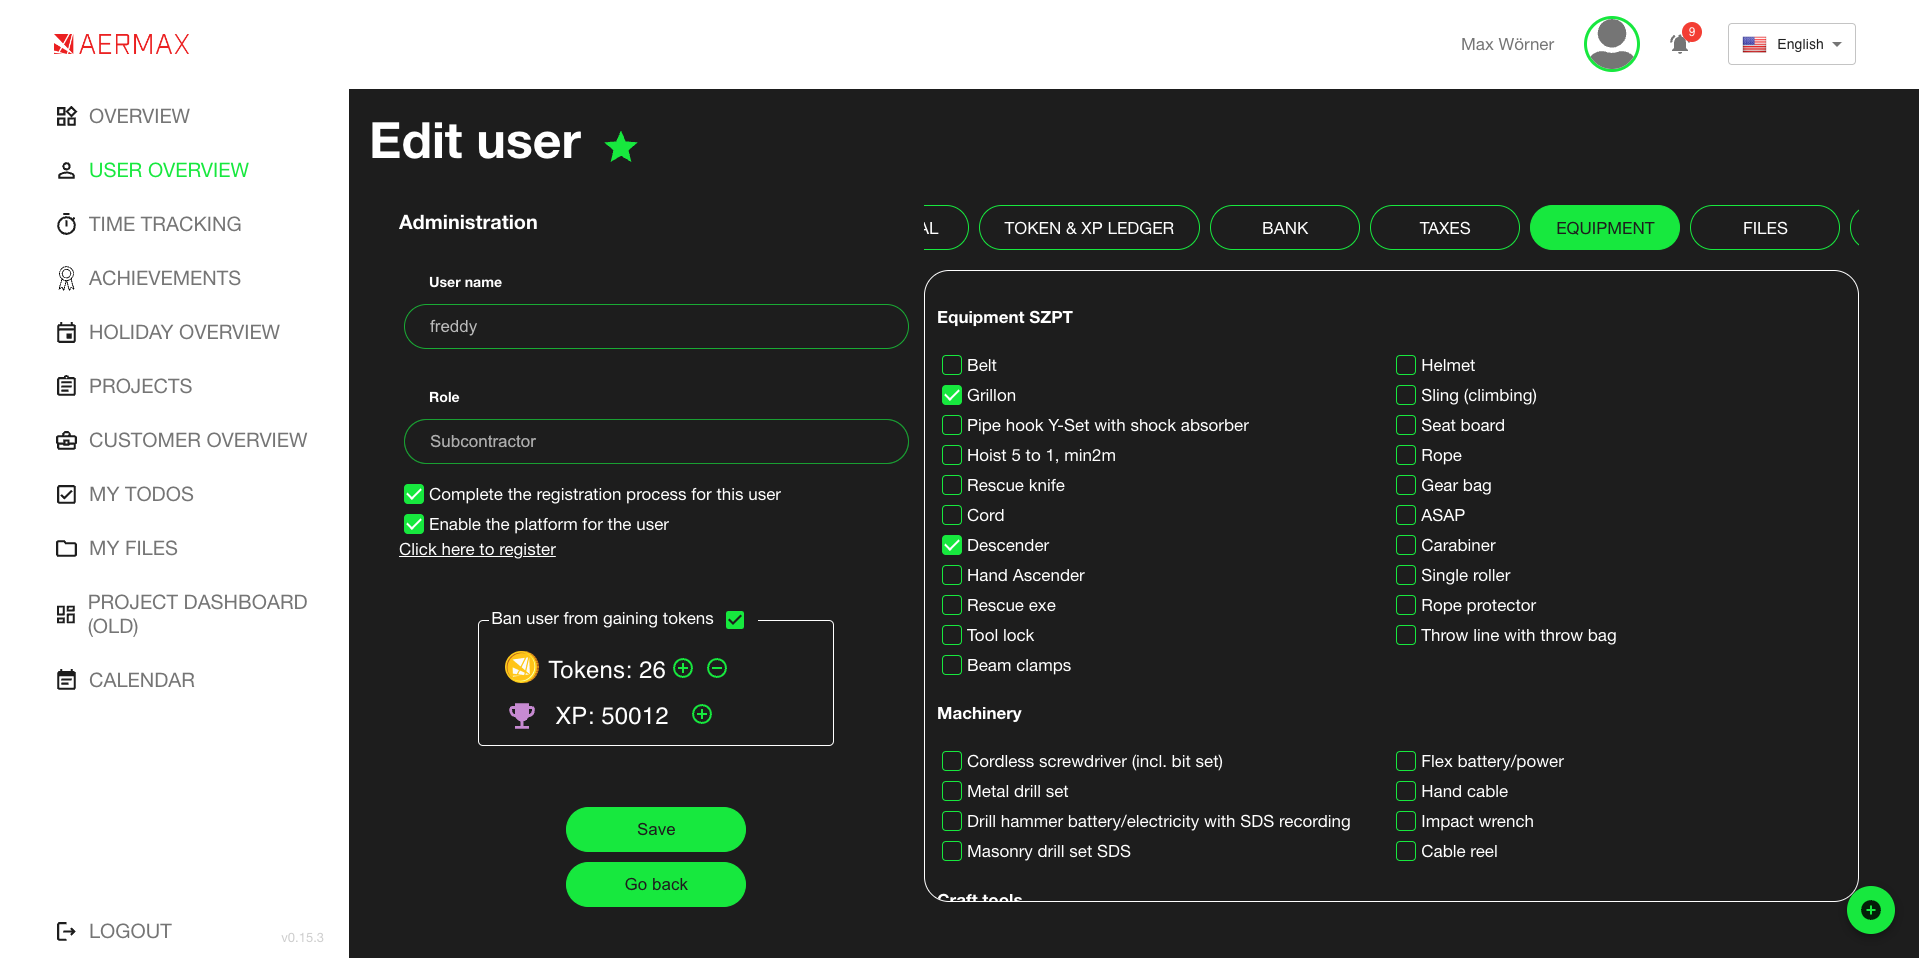
\includegraphics{src/assets/chapters/StaticDynamicEquipementList.png}
    }
    \caption{Previous Static Equipment List}
    \label{fig:static_equipment_list}
\end{figure}

\subsubsection{Dynamic Equipment List solution}
To address these issues, we are transitioning to a dynamic equipment list. The dynamic implementation will automatically update the list based on changes in the equipment database, ensuring real-time accuracy and reducing maintenance overhead. Key features of the dynamic implementation include:
\begin{itemize}
    \item \textbf{Real-time Updates:} The list will automatically reflect changes made to the equipment database.
    \item \textbf{Improved Scalability:} The system can handle an increased number of equipment items without additional maintenance.
    \item \textbf{Enhanced User Experience:} Users will have access to up-to-date information, improving their ability to make decisions.
    \item \textbf{Reduced Maintenance:} Eliminates the need for manual updates, reducing the time and effort required to maintain the list.
    \item \textbf{Request System:} Subcontractors can request new equipment items directly through the system, allowing admins to approve, reject, and assign these items to appropriate groups.
\end{itemize}

The planned dynamic equipment list will also include comprehensive admin and subcompany views. As shown in Figure \ref{fig:dynamic_equipment_list_admin}, admins will have the capability to create groups, assign equipment, move equipment, and approve or reject equipment requests. Subcontractors, as illustrated in Figure \ref{fig:dynamic_equipment_list_subcompany}, will be able to write and request new equipment items, ensuring they have the necessary tools for their projects.

\begin{figure}[H]
    \centering
    \resizebox{1\textwidth}{!}{
        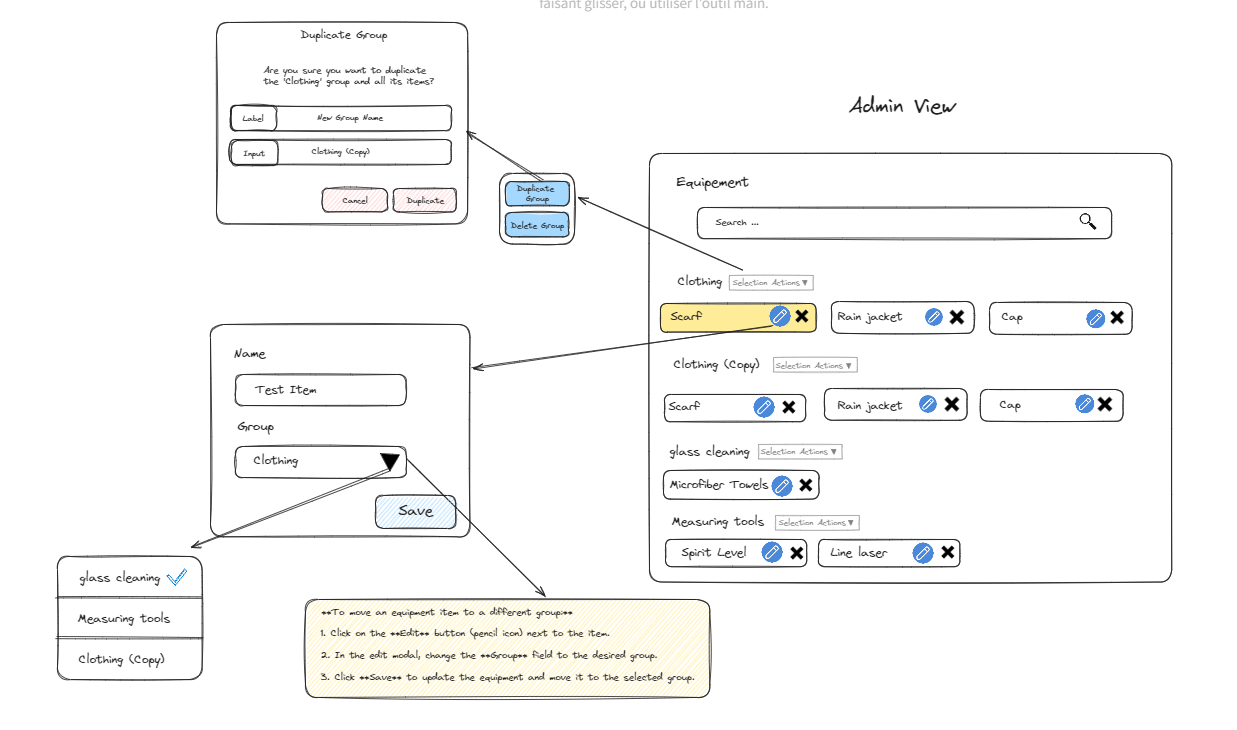
\includegraphics{src/assets/chapters/DynamicEquipementAdmin.PNG}
    }
    \caption{Planned Dynamic Equipment List - Admin View}
    \label{fig:dynamic_equipment_list_admin}
\end{figure}

\begin{figure}[H]
    \centering
    \resizebox{1\textwidth}{!}{
        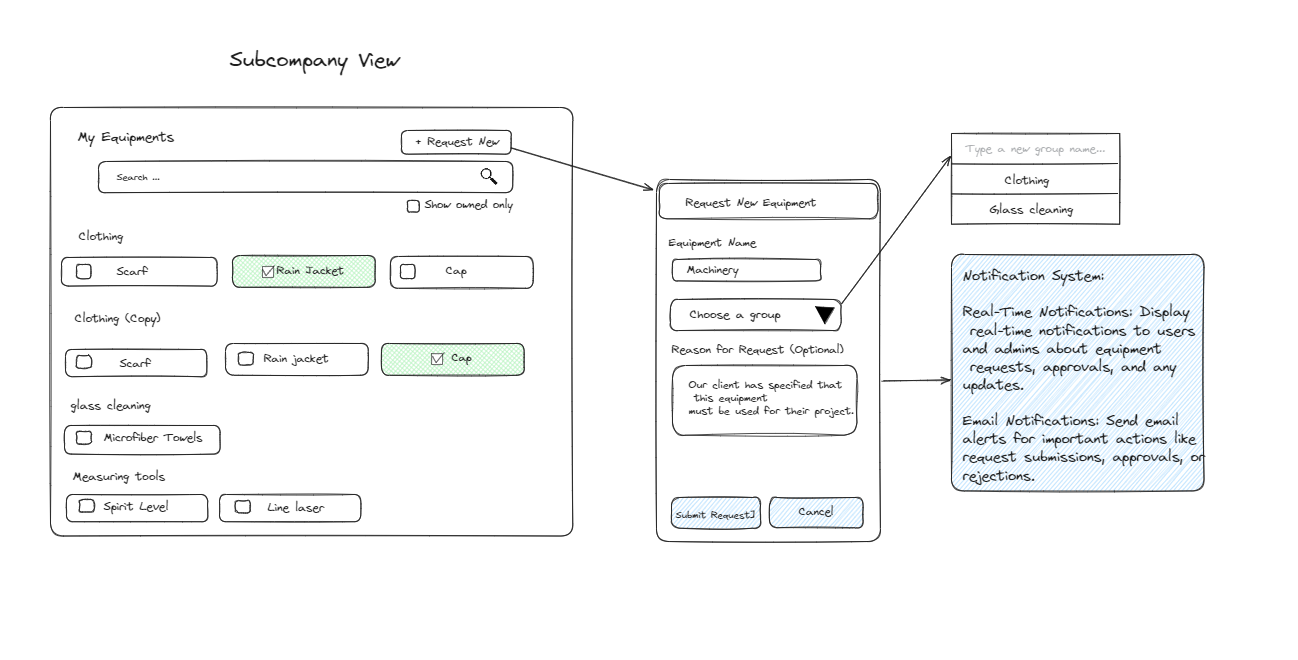
\includegraphics{src/assets/chapters/DynamicEquipementSubcompany.PNG}
    }
    \caption{Planned Dynamic Equipment List - Subcompany View}
    \label{fig:dynamic_equipment_list_subcompany}
\end{figure}

\subsubsection{Dynamic Equipment Design}
To effectively transition from a static to a dynamic equipment list, we need to carefully design the system architecture. The dynamic system will facilitate real-time updates, scalability, and a user-friendly experience. The following sections provide a detailed overview of the class structure and interactions essential for implementing this dynamic equipment list.

The dynamic equipment list system will consist of several key components:

\begin{itemize}
    \item \textbf{Equipment Class:} This class will represent individual equipment items, including attributes such as name, group, status (requested, approved, rejected), and other relevant details.
    \item \textbf{Group Class:} This class will manage groups of equipment, allowing the creation, duplication, and deletion of groups. It will also handle the assignment and movement of equipment items between groups.
    \item \textbf{Request Class:} This class will handle equipment requests submitted by subcontractors. It will track the status of requests (pending, approved, rejected) and include details such as the equipment name and requested group.
    \item \textbf{User Class:} This class will manage user information, differentiating between admin and subcontractor roles, and providing appropriate permissions and functionalities for each role.
    \item \textbf{Notification System:} This component will handle real-time and email notifications to keep users informed about important actions like equipment requests, approvals, and rejections.
\end{itemize}
\paragraph{Class Diagram}
The class diagram below illustrates the key components and relationships involved in the dynamic equipment list feature.

\begin{figure}[H]
    \centering
    \resizebox{1\textwidth}{!}{
        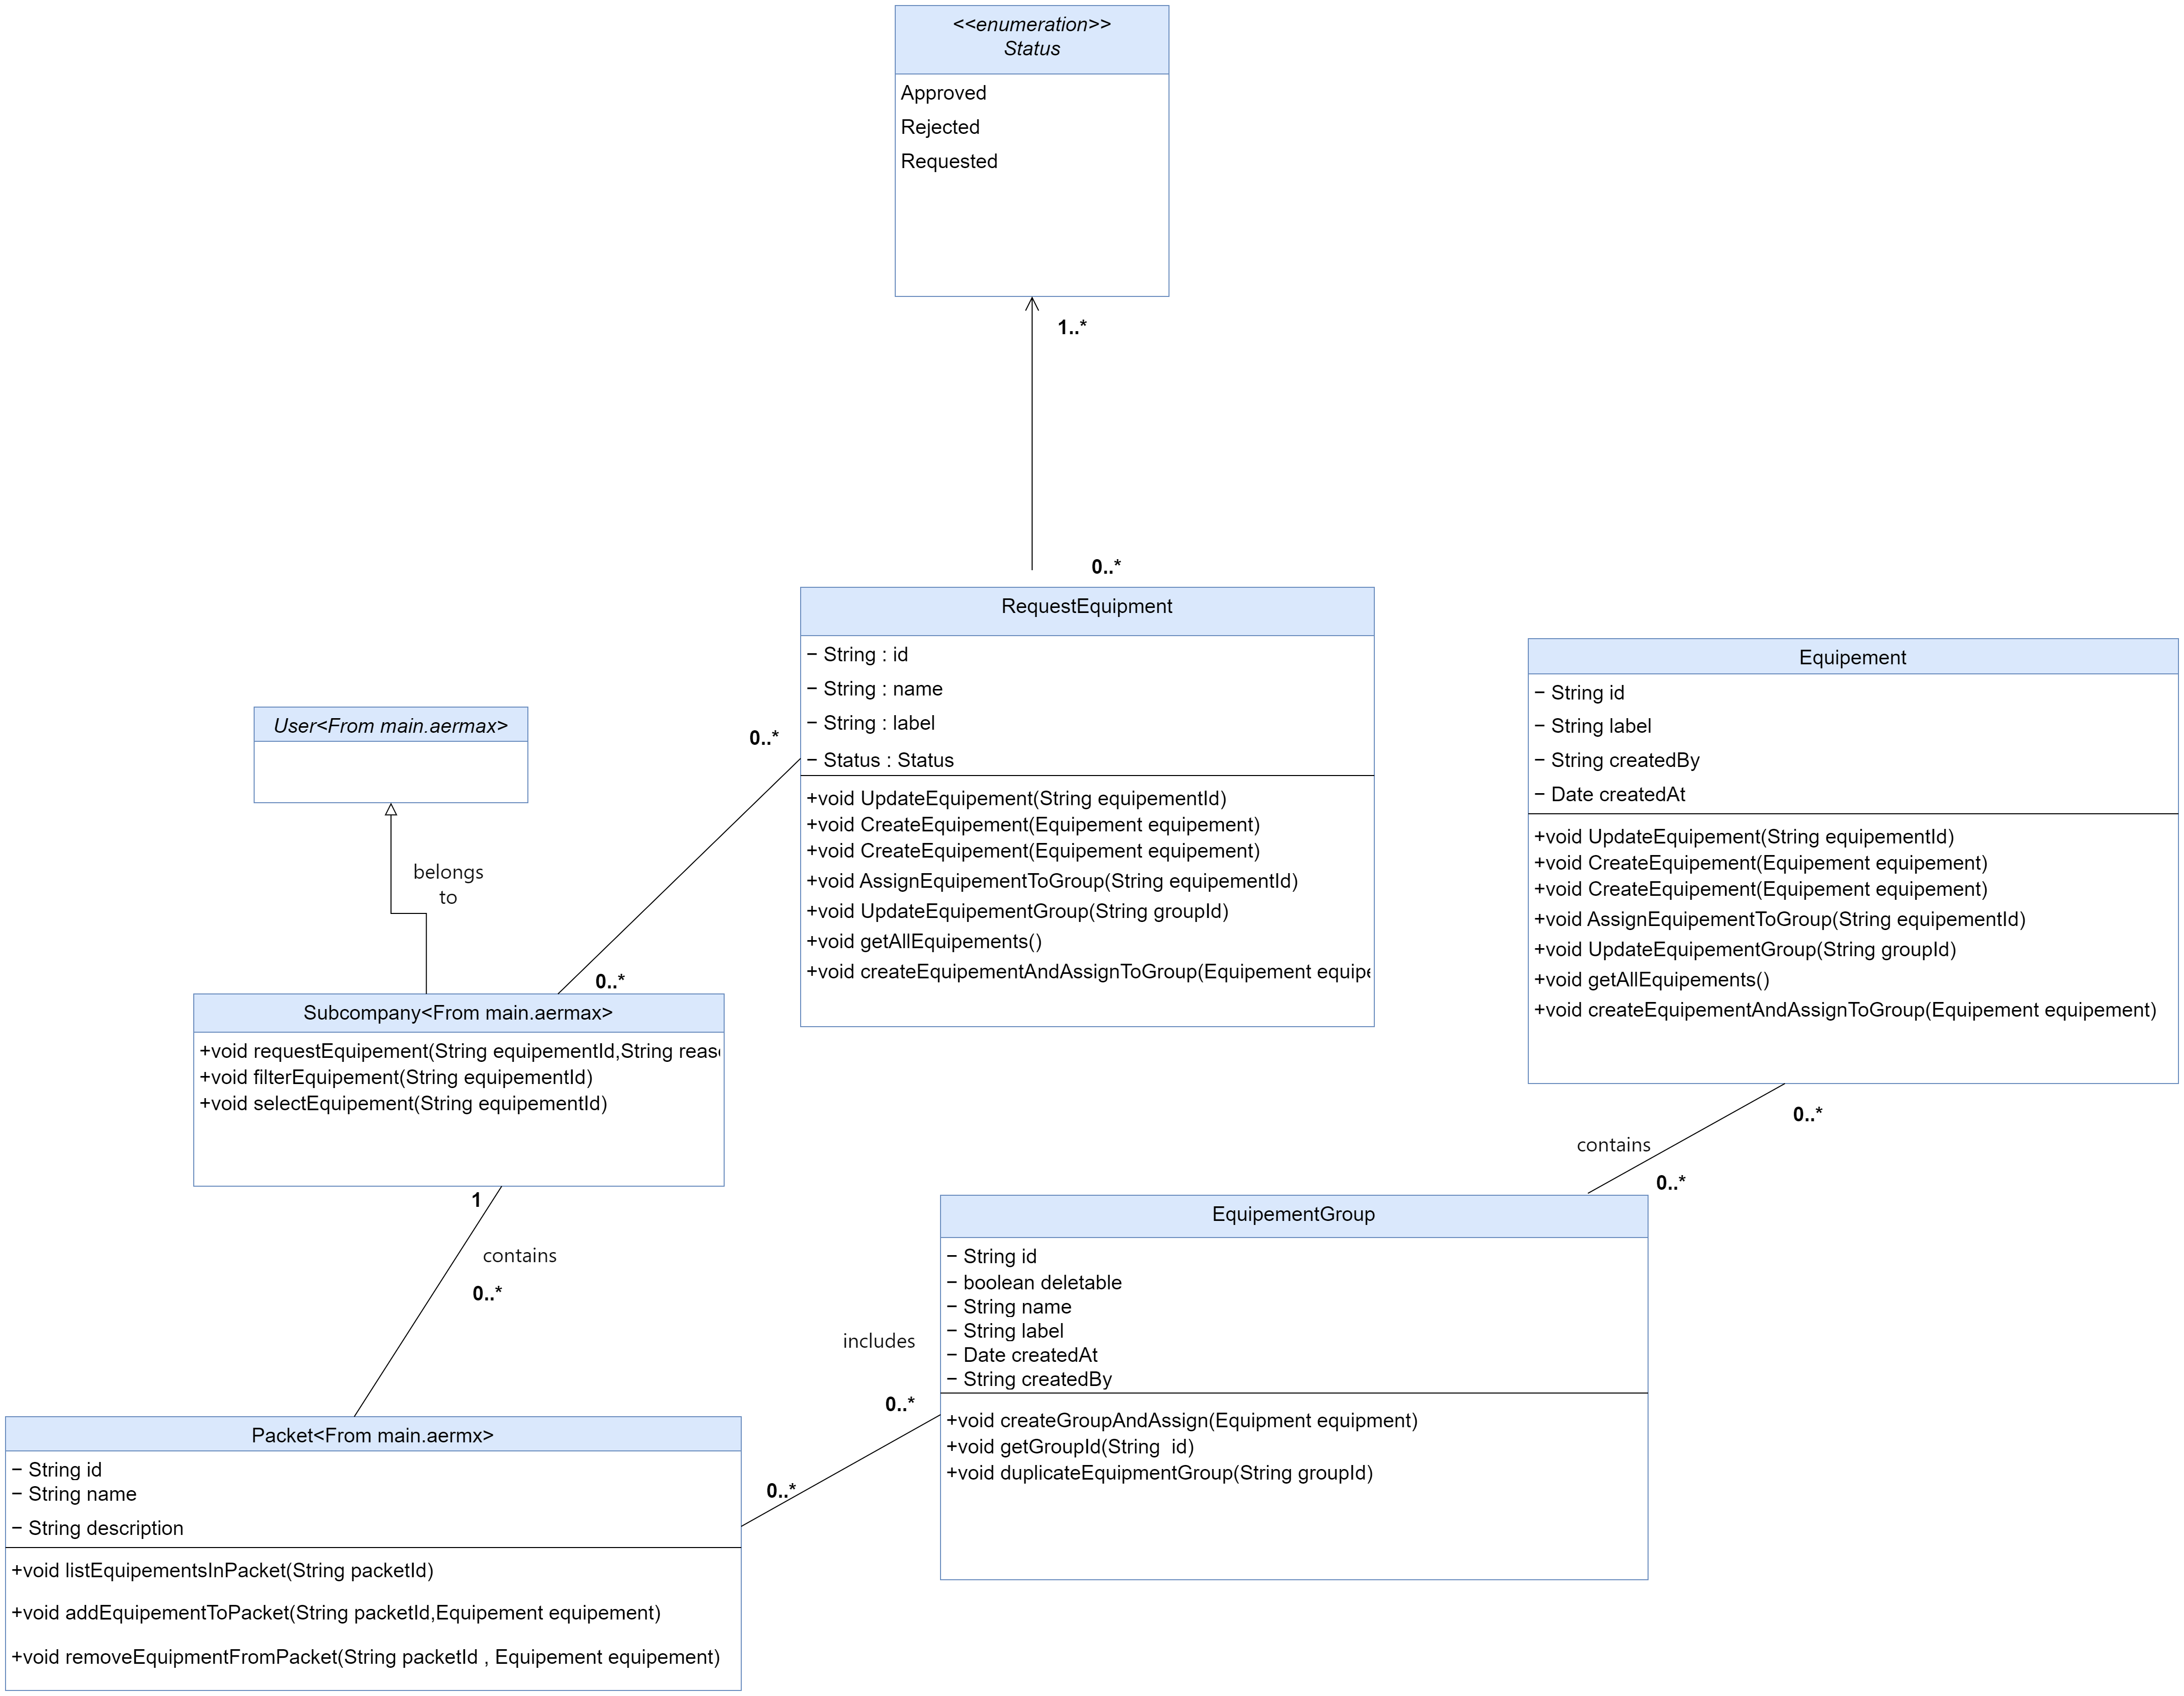
\includegraphics{src/assets/diagrams/DynamiEquipementListPng.png}
    }
    \caption{Class Diagram for Dynamic Equipment List}
    \label{fig:class_diagram}
\end{figure}


\paragraph{Subcompany Interface}
The images below show the subcompany interface after the implementation of the dynamic equipment list, illustrating the improved user experience for subcompany users.

\begin{figure}[H]
\centering
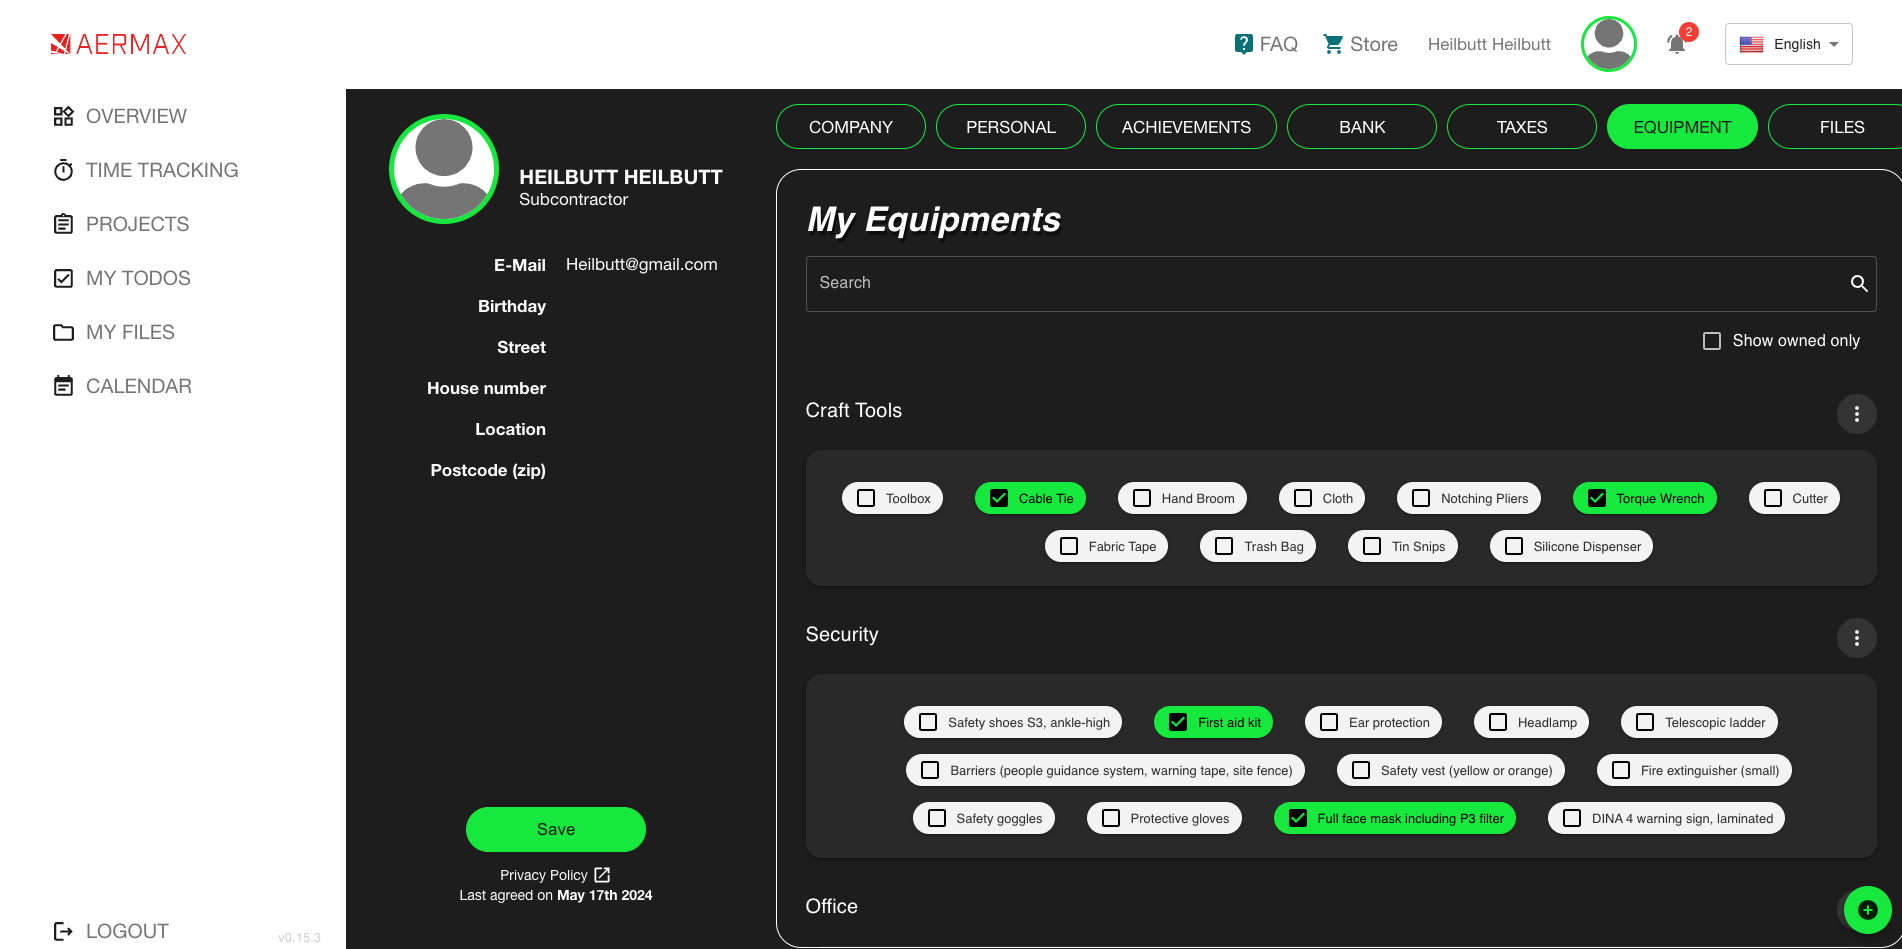
\includegraphics[width=0.9\textwidth]{src/assets/images/Interface1.png}
\caption{Subcompany Interface - Viewing Assigned Equipment}
\label{fig:subcompany_interface_1}
\end{figure}

\subsection{Adjust Feedback Notification}
To enhance the feedback feature, we plan to implement a system that allows administrators to send feedback notifications directly to Microsoft Teams. This feature aims to streamline communication and ensure that feedback is promptly addressed. The following sections outline the implementation strategy for this feature.

The feedback system will consist of several key components:

\begin{itemize}
    \item \textbf{Feedback Form:} The user interface where administrators can submit feedback. The form will include options for categorizing the feedback (Error, Incomprehensible, Unwanted Behavior, Miscellaneous) and a text area for detailed descriptions.
    \item \textbf{Feedback Database:} A storage system to save feedback entries. Each entry will include the feedback category, description, and a timestamp.
    \item \textbf{Notification Service:} A backend service that processes feedback entries and sends notifications to Microsoft Teams. This service will be designed to be extendable, allowing for future integration with other communication channels such as Slack or email.
\end{itemize}

\paragraph{Implementation Steps}
\begin{enumerate}
    \item \textbf{Feedback Form UI:} Enhance the existing feedback form (Figure \ref{fig:feedback_form}) to include the necessary fields and submission button. Ensure the form captures the feedback category and description.
    \item \textbf{Database Integration:} Create or update the database schema to store feedback entries. Each entry should capture the feedback category, description, and a timestamp.
    \item \textbf{Notification Service:} Develop a backend service that listens for new feedback entries in the database. Upon detecting a new entry, the service will format the feedback and send it as a notification to a designated Microsoft Teams channel.
    \item \textbf{Microsoft Teams Integration:} Use the Microsoft Teams API to send notifications. Ensure the notifications include all relevant feedback details and are formatted for readability.
\end{enumerate}

The following image (Figure \ref{fig:feedback_form}) illustrates the user interface for submitting feedback.

\begin{figure}[H]
    \centering
    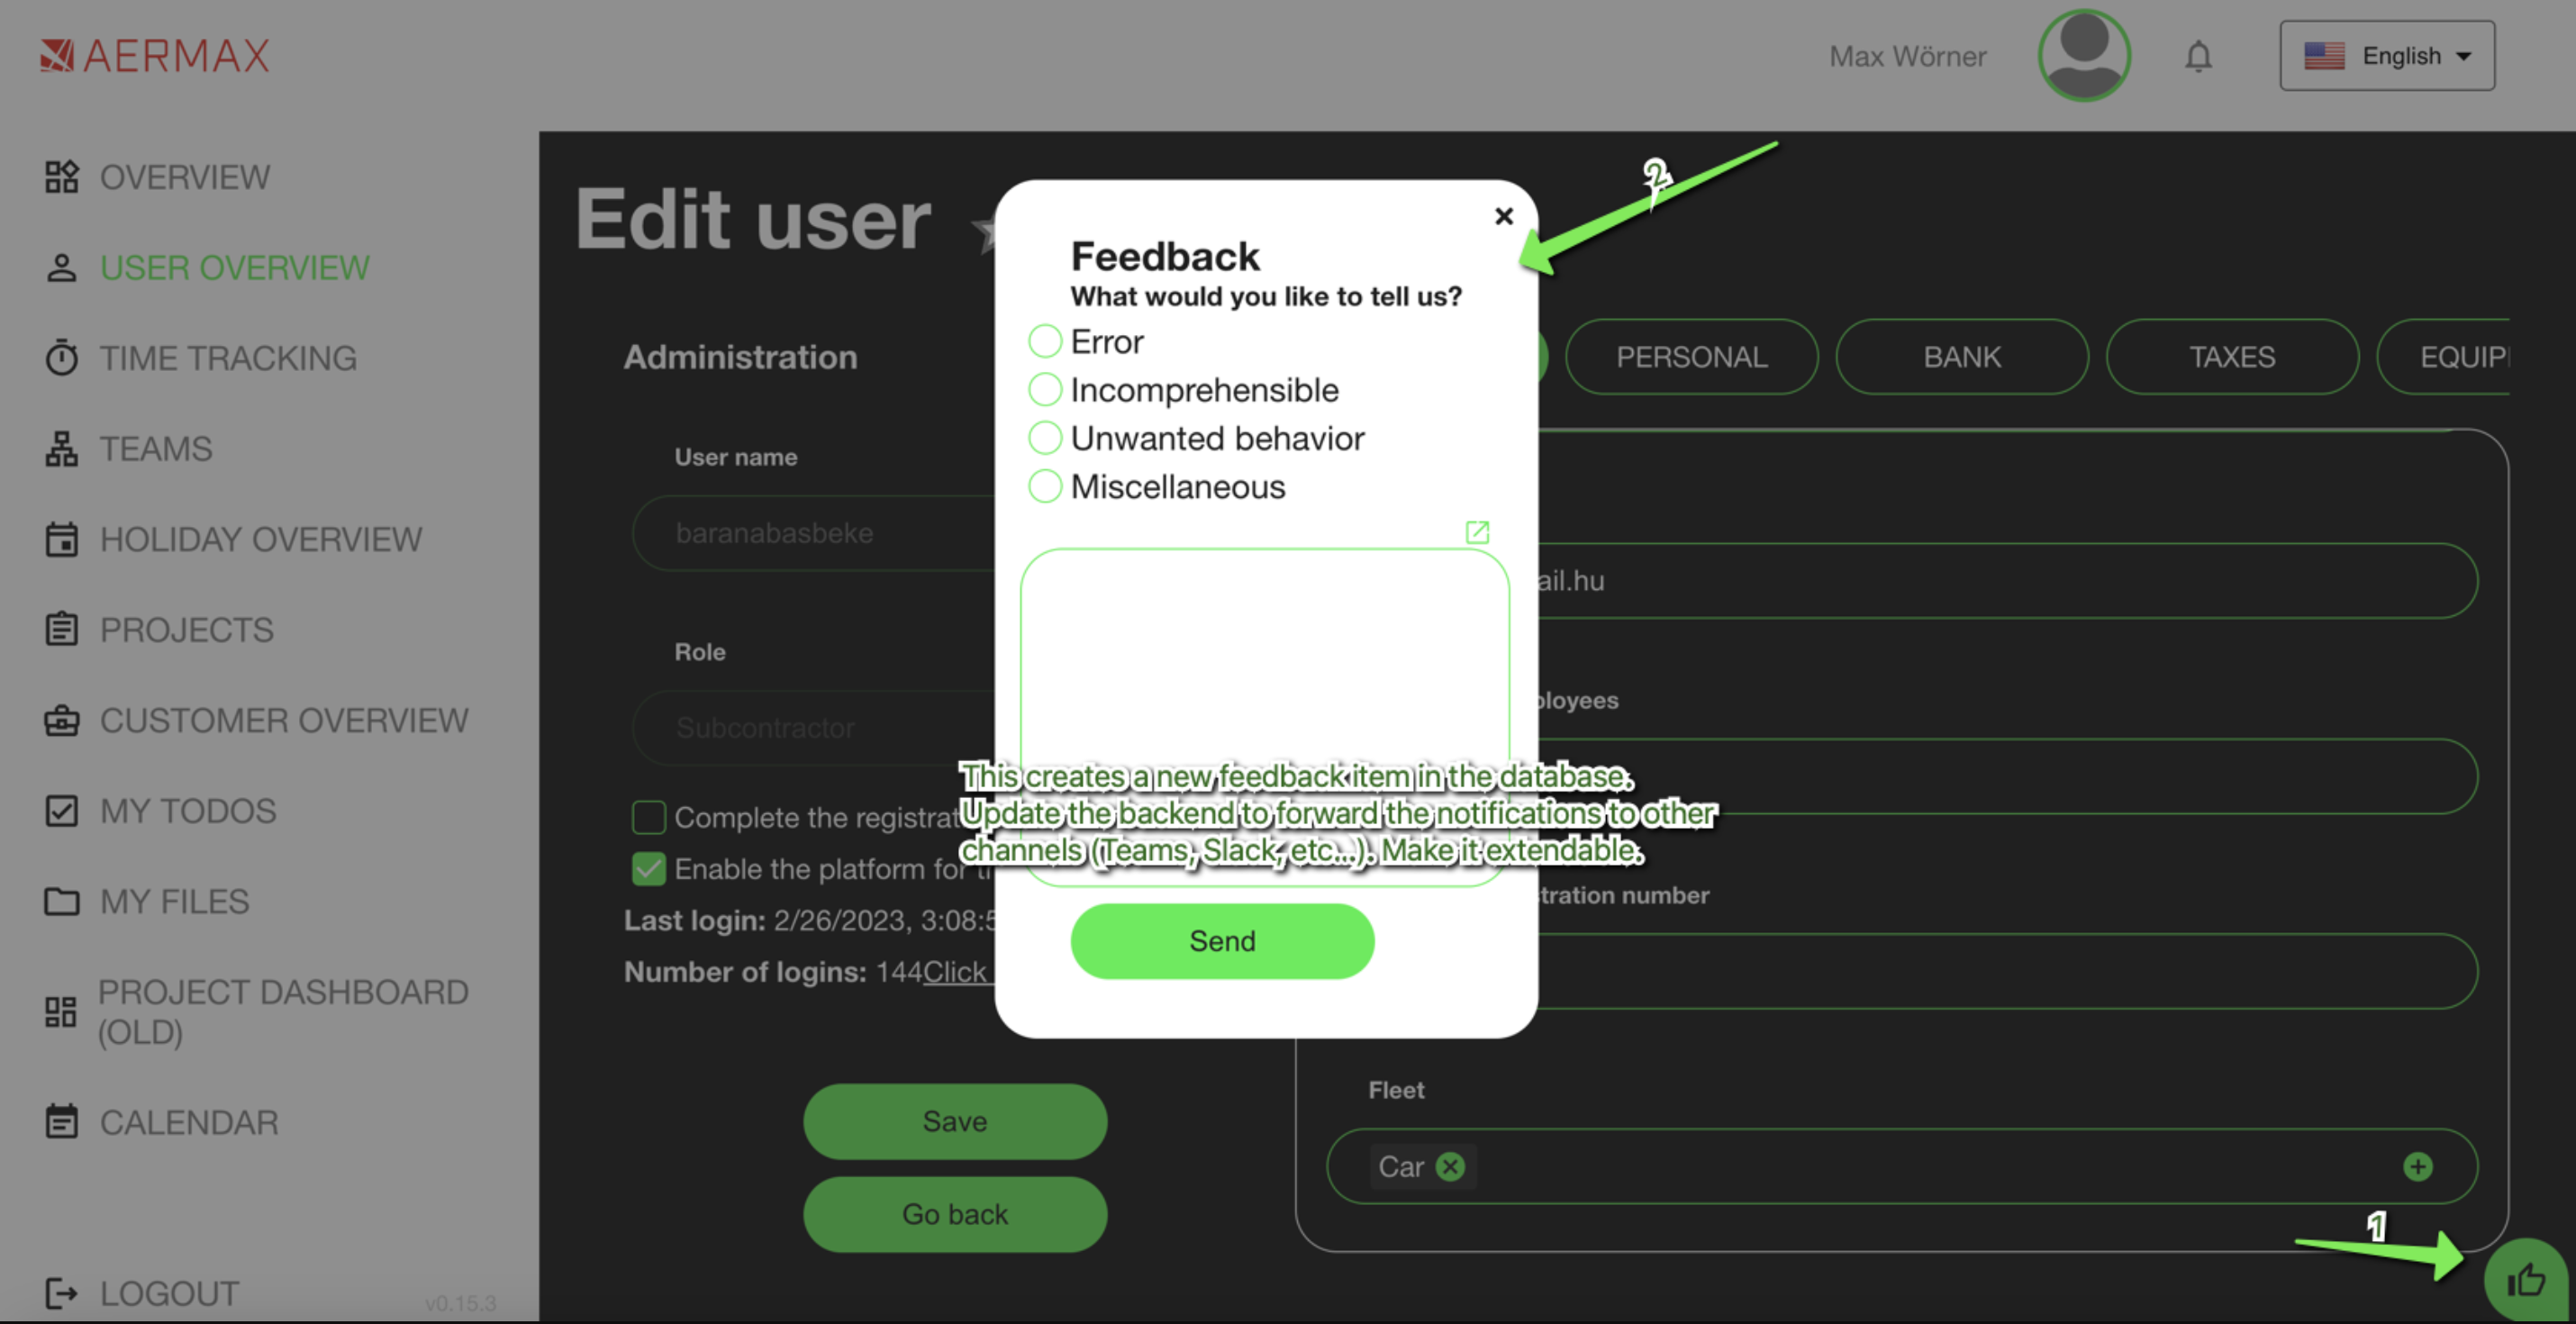
\includegraphics[width=1\textwidth]{src/assets/images/TeamsNotification.png}
    \caption{Feedback Form and Notification}
    \label{fig:feedback_form}
\end{figure}

\subsection{Overhaul of the Role System}
The Aermax platform's role system was overhauled during Sprint 1 to improve clarity and security. Previously, roles had overlapping permissions, causing confusion and security issues. Now, each role has specific permissions aligned with its responsibilities.

\subsubsection{Detailed Role Permissions Before \& After}
\begin{longtable}{|p{3cm}|p{5cm}|p{5cm}|}
\caption{Comparison of role permissions before and after the overhaul.} \label{tab:role_permissions_comparison} \\
\hline
\textbf{Role} & \textbf{Permissions Before Overhaul} & \textbf{Permissions After Overhaul} \\ \hline
\endfirsthead

\multicolumn{3}{c}%
{{\bfseries Table \thetable\ Continued from previous page}} \\
\hline
\textbf{Role} & \textbf{Permissions Before Overhaul} & \textbf{Permissions After Overhaul} \\ \hline
\endhead

\hline \multicolumn{3}{|r|}{{Continued on next page}} \\ \hline
\endfoot

\hline
\endlastfoot

Administrator & 
- Limited access to projects managed by non-admin Project Managers &
- Full access to all projects \\ \hline

Worker & 
- Could see all project packets &
- Can only see their own projects and packets \\ \hline


Team Leader & 
- Could see only their own packets &
- Can see packets of other workers within their phase   \\ \hline

\end{longtable}

\textbf{Scenario Demonstrations After Overhaul:}
\begin{itemize}
    \item \textbf{Administrator Scenario:} An Administrator maintains complete control, capable of managing all aspects of the project lifecycle.
    \item \textbf{Project Manager Scenario:} Project Managers are now provided with tailored access, capable of managing specific project packets and workflows.
    \item \textbf{Worker Scenario:} Workers are limited to their own packets, focusing their dashboard on personal tasks without additional project creation or overview privileges.
    \item \textbf{Team Leader Scenario:} Team Leaders have targeted oversight, managing only the packets within their project phase, without the distraction of other project overviews or creation capabilities.
\end{itemize}
This targeted approach in the role system refines the user experience on the Aermax platform, ensuring each role has the access needed to perform effectively, securely, and efficiently.

\subsection{Enhance Working Packets UI \& UX}
In our continuous efforts to elevate the user experience on the Aermax platform, a significant upgrade was made to the Working Packets UI \& UX, particularly focusing on the administrative interface. Key improvements include:

\begin{itemize}
    \item Alleviating the difficulties the admin faced in managing packets.
    \item Addressing the need to duplicate each packet individually when 30 packets needed duplication in one day.
    \item Developing a new interface presented as a table.
    \item Allowing the admin to duplicate multiple packets simultaneously.
    \item Offering more filtering functionalities.
    \item Providing an improved, user-friendly view.
\end{itemize}

See the implemented feature in Figure \ref{fig:ui_ux_enhancements}.

\begin{figure}[H]
    \centering
    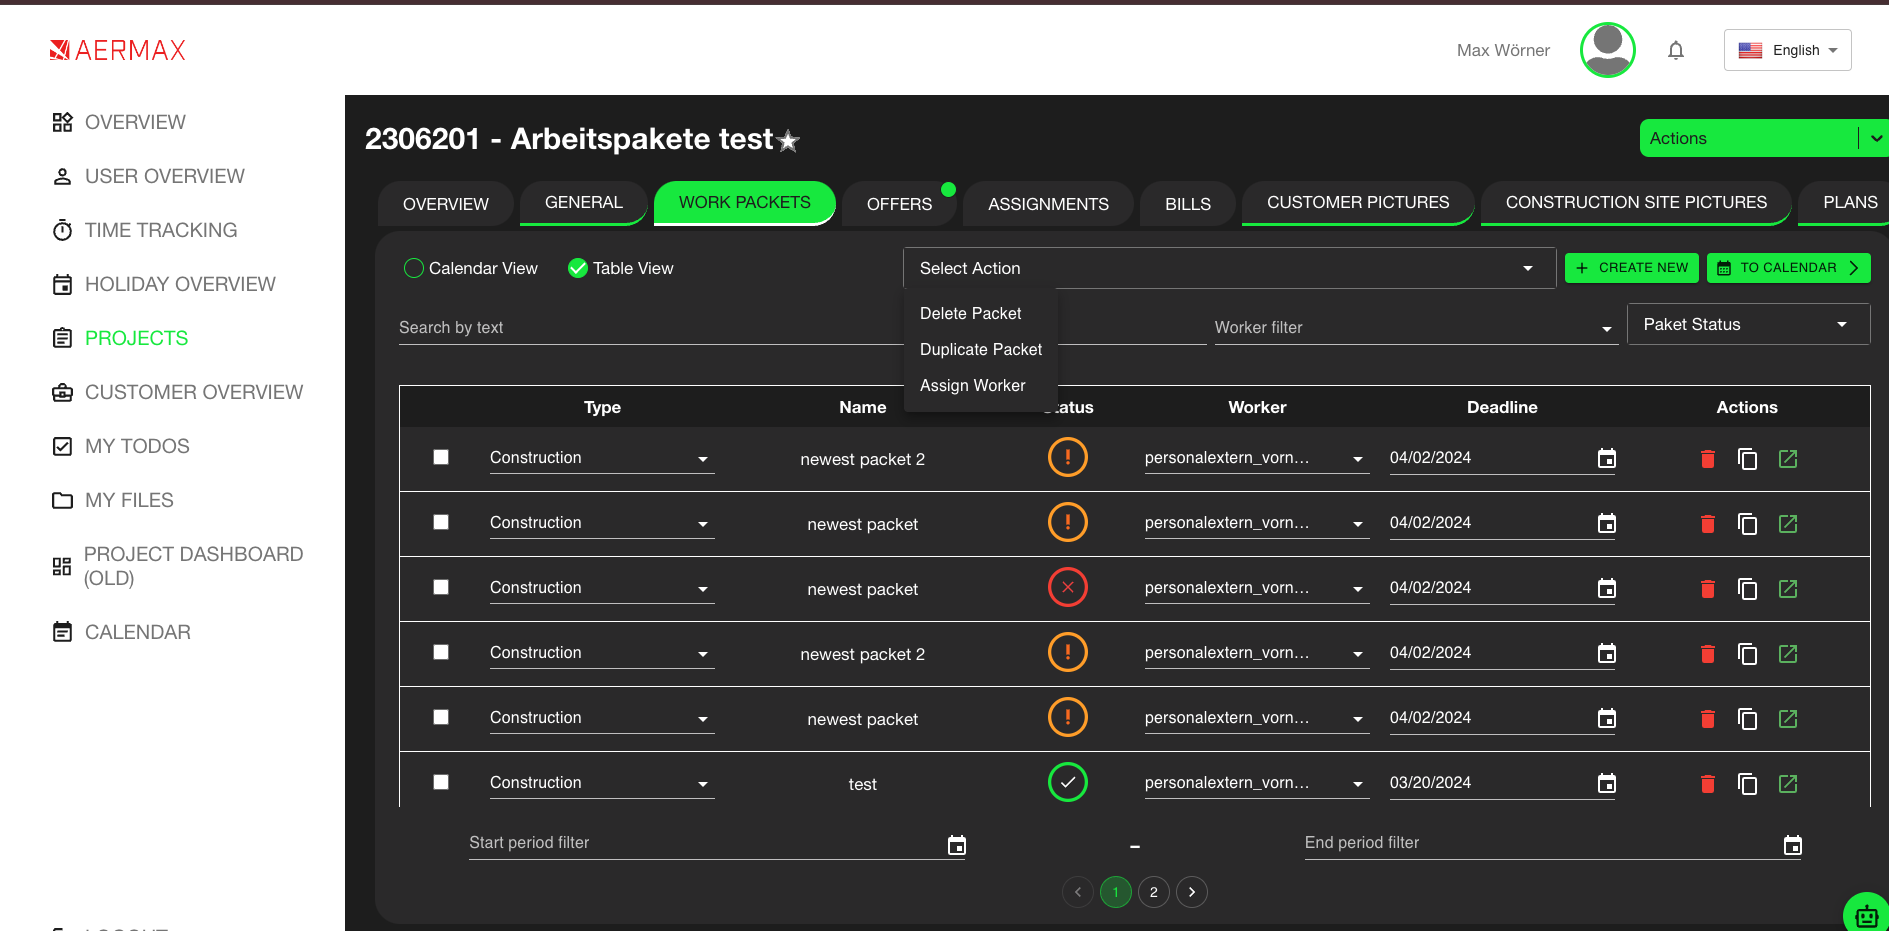
\includegraphics[width=0.9\textwidth]{src/assets/chapters/newTable2.png}
    \caption{Sketch of Planned UI/UX Enhancements for Working Packets}
    \label{fig:ui_ux_enhancements}
\end{figure}

\subsection{User Authentication System}
We implemented an authentication system using Keycloak. As part of this overhaul, we encountered the challenge of duplicate user entries due to previous system design limitations. By leveraging Keycloak’s versatile user federation and identity provider features, we were able to consolidate user accounts and eliminate redundancies, thereby solving the issue of duplicate entries. Keycloakify complemented this integration by allowing us to customize the authentication pages to align with our platform's aesthetics and usability standards.

\subsubsection{Feature Implementation Table:}
\begin{table}[H]
\centering
\begin{tabularx}{\textwidth}{|X|X|X|}
\hline
\textbf{Feature} & \textbf{Technology Implemented} & \textbf{Description} \\
\hline
Login/Signup & Keycloak, Keycloakify & Integrated with Keycloak to secure and streamline user access, enhanced by Keycloakify for customized UI/UX. \\
\hline
Password Management & Keycloak & Developed a secure and user-friendly password management system, providing users with ease of control over their credentials. \\
\hline
\end{tabularx}
\caption{Summary of Keycloak feature implementations.}
\label{tab:keycloak_features}
\end{table}

\setcounter{secnumdepth}{0}
\section{Conclusion}
Sprint 1 has laid a strong foundation for the Aermax platform by addressing critical needs and improving overall functionality and user experience. Looking ahead to Sprint 2, we will focus on a major feature: the reward system, which promises to further enhance user engagement and satisfaction.

